\chapter{EXPERIMENTO}
\label{chap:experimento}

Para aplicar os conceitos visto na seção \ref{chap:estudo}, foi proposto um desafio em que consiste medir o tempo de voo de um helicóptero de papel. Para a concepção do helicóptero foi utilizado o modelo proposto pela metodologia \textit{SixSigma}, conforme visto na Figura \ref{fig:model_heli}. 

\begin{figure}[H]
  \caption{Modelo do helicóptero de papel.}
  \centering
  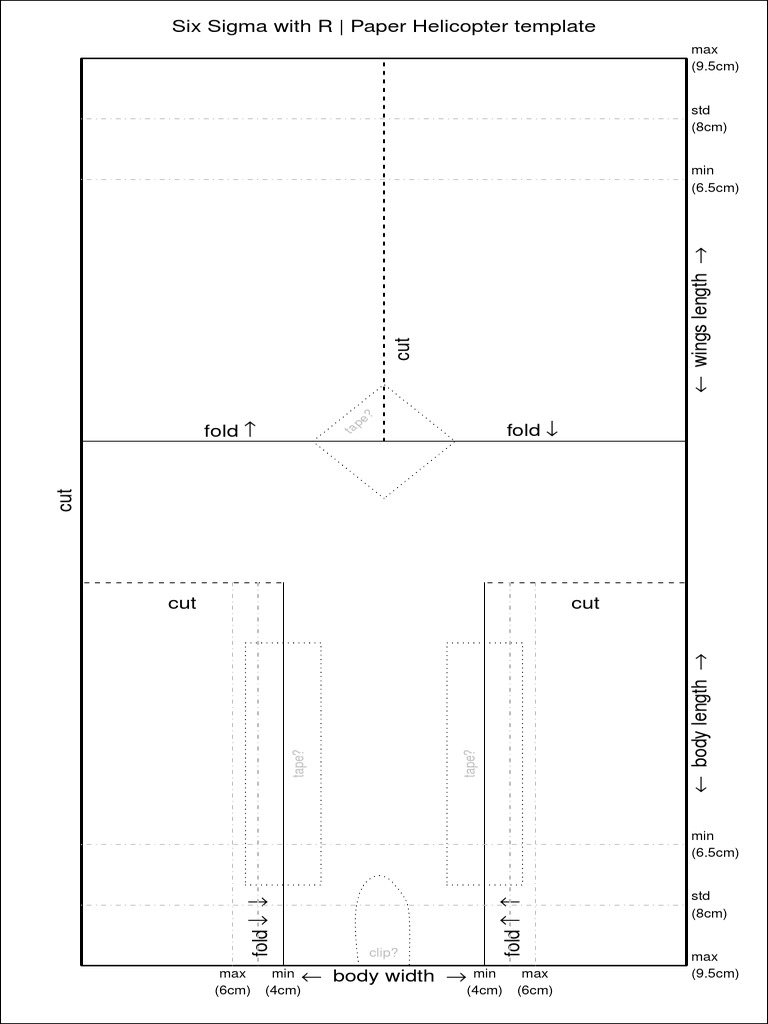
\includegraphics[width=0.7\textwidth]{images/helicopter.jpeg}
  \label{fig:model_heli}
\end{figure}

Após as dobras e cortes recomendados pelo \textit{template}, o protótipo obtido como configuração inicial para análise do estudo pode ser visto na Figura \ref{fig:heli_papel}.

\begin{figure}[H]
  \caption{Helicóptero de papel.}
  \centering
  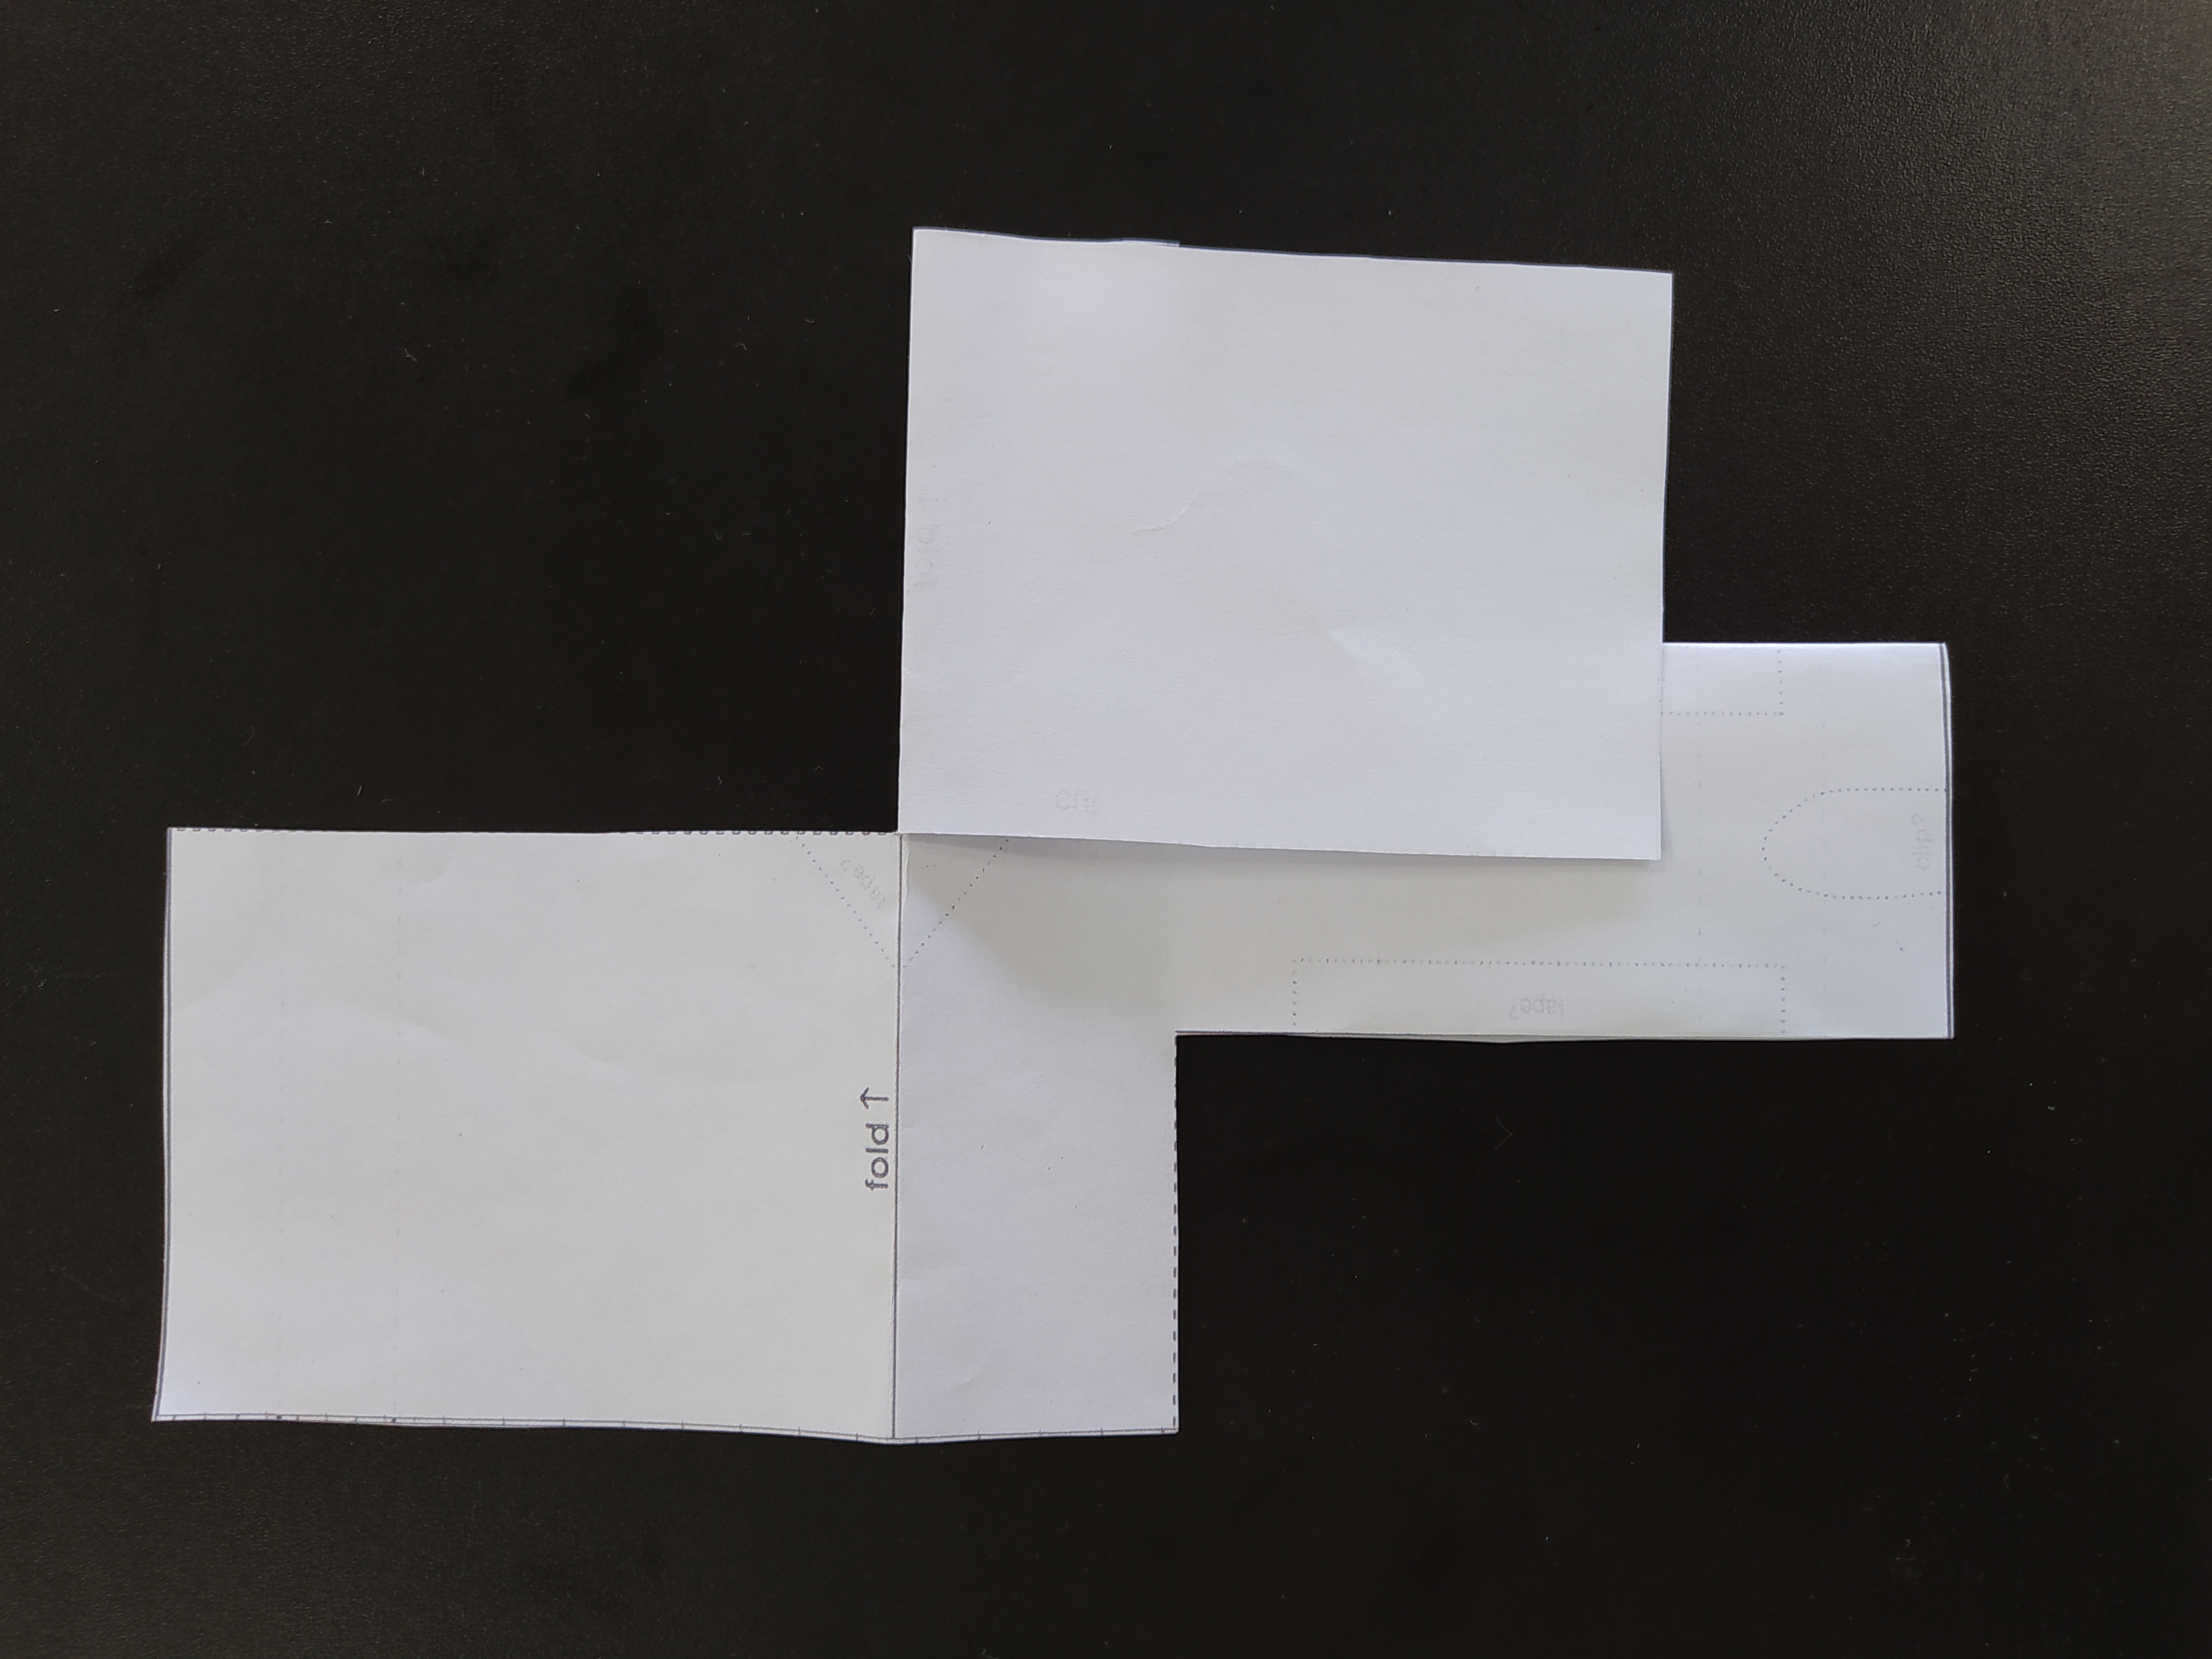
\includegraphics[width=1\textwidth]{images/IMG_20200918_162251.jpg}
  \caption*{Fonte: Autoria própria.}
  \label{fig:heli_papel}
\end{figure}

Para obter-se o melhor helicóptero, ou seja, aquele que apresente o maior tempo de voo, foi considerado alguns fatores para alterar sua configuração inicial como pode ser visto na tabela \ref{tab:fatores}. Por fim, foi realizado os testes, medição do tempo de voo, para cada possível combinação dos fatores.


\begin{table}[H]
  \caption{Fatores considerados para alterar a estrutura.}
  \centering
  \begin{tabular}{|c|c|c|}
  \hline
  \rowcolor[HTML]{EFEFEF} 
  \textbf{Fatores}      & \textbf{Configuração atual} & \textbf{Alteração permitida} \\ \hline
  Clipe                 & Não                         & Sim                          \\ \hline
  \rowcolor[HTML]{EFEFEF} 
  Altura (m)            & 1,30                        & 2,10                         \\ \hline
  Adesivo (Asa)         & Não                         & Sim                          \\ \hline
  \rowcolor[HTML]{EFEFEF} 
  Fita (Corpo/Esquerdo) & Não                         & Sim                          \\ \hline
  Fita (Corpo/Direito)  & Não                         & Sim                          \\ \hline
  \end{tabular}
  \caption*{Autoria própria.}
  \label{tab:fatores}
  \end{table}
